% Plain-language diagrams of the L2 layer (one diagram per page).
% Build: tectonic l2_steps.tex  ->  l2_steps.pdf (used by the report and the slides)
\documentclass[tikz,border=10pt]{standalone}
\usepackage{fontspec}
\renewcommand{\familydefault}{\sfdefault}
\usepackage{amsmath,amssymb}
\usetikzlibrary{arrows.meta,positioning,calc,fit,backgrounds,decorations.pathreplacing,shapes.geometric}
\definecolor{lblue}{HTML}{2A78D6}
\definecolor{lsoft}{HTML}{E6F0FB}
\definecolor{lorange}{HTML}{EB6834}
\definecolor{lgreen}{HTML}{1F7A46}
\definecolor{lred}{HTML}{B83227}
\definecolor{ink}{HTML}{1B2430}
\definecolor{muted}{HTML}{5A6472}
\definecolor{tint}{HTML}{EEF2F6}
\definecolor{r1}{HTML}{2A78D6}
\definecolor{r2}{HTML}{7B4FB8}
\definecolor{r3}{HTML}{1F8A80}
\definecolor{r4}{HTML}{C2185B}
\tikzset{
  >={Stealth[length=2.6mm]},
  box/.style={draw=ink,thick,rounded corners=4pt,fill=white,align=center,inner sep=6pt,font=\small},
  soft/.style={box,draw=lblue,fill=lsoft},
  lab/.style={font=\footnotesize,color=muted,align=center},
  rev/.style={circle,draw=#1,very thick,fill=#1!12,minimum size=1.05cm,font=\small\bfseries,text=ink},
  flow/.style={->,thick,ink},
  talk/.style={<->,thick,dashed,lblue},
  step/.style={circle,fill=ink,text=white,font=\footnotesize\bfseries,inner sep=1.5pt,minimum size=0.5cm},
}

\begin{document}

% ------------------------------------------------------------------ 1 committee overview
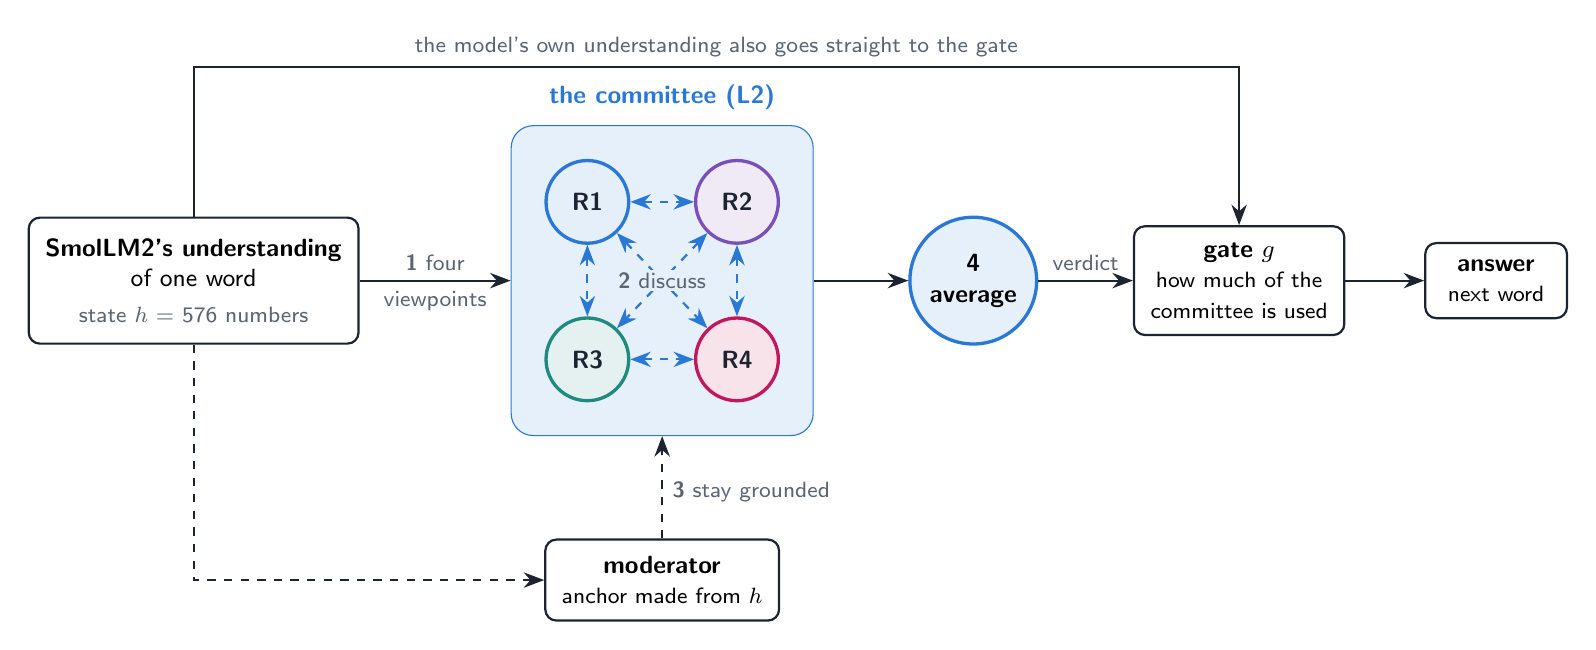
\begin{tikzpicture}
  \node[box,minimum width=3.0cm,minimum height=1.6cm] (h) at (0,0) {\textbf{SmolLM2's understanding}\\of one word\\[2pt]{\footnotesize\color{muted}state $h$ = 576 numbers}};
  % committee
  \node[rev=r1] (a) at (5.0,1.0) {R1};
  \node[rev=r2] (b) at (6.9,1.0) {R2};
  \node[rev=r3] (c) at (5.0,-1.0) {R3};
  \node[rev=r4] (d) at (6.9,-1.0) {R4};
  \draw[talk] (a) -- (b); \draw[talk] (c) -- (d); \draw[talk] (a) -- (c); \draw[talk] (b) -- (d);
  \draw[talk] (a) -- (d); \draw[talk] (b) -- (c);
  \begin{scope}[on background layer]
    \node[draw=lblue,fill=lsoft,rounded corners=8pt,inner sep=12pt,fit=(a)(b)(c)(d)] (com) {};
  \end{scope}
  \node[font=\small\bfseries,color=lblue,above=2pt of com] {the committee (L2)};
  \draw[flow] (h.east) -- node[above,lab]{\textbf{1} four}node[below,lab]{viewpoints} (com.west);
  % moderator
  \node[box,minimum width=2.6cm,below=1.3cm of com] (mod) {\textbf{moderator}\\{\footnotesize anchor made from $h$}};
  \draw[->,thick,dashed,ink] (mod.north) -- node[right,lab,pos=0.45]{\textbf{3} stay grounded} (com.south);
  \draw[->,thick,dashed,ink] (h.south) |- (mod.west);
  \node[lab,align=center] at (5.95,0) {};
  \node[lab,fill=lsoft,inner sep=1pt] at (5.95,0.0) {\textbf{2} discuss};
  % verdict
  \node[circle,draw=lblue,very thick,fill=lsoft,minimum size=1.3cm,font=\small\bfseries,align=center,right=1.2cm of com] (avg) {\textbf{4}\\average};
  \draw[flow] (com.east) -- (avg);
  % gate
  \node[box,minimum width=2.4cm,right=1.2cm of avg] (gate) {\textbf{gate} $g$\\{\footnotesize how much of the}\\{\footnotesize committee is used}};
  \draw[flow] (avg) -- node[above,lab]{verdict} (gate);
  \draw[flow] (h.north) -- ++(0,1.9) -| node[pos=0.25,above,lab]{the model's own understanding also goes straight to the gate} (gate.north);
  \node[box,right=1.0cm of gate,minimum width=1.8cm] (ans) {\textbf{answer}\\{\footnotesize next word}};
  \draw[flow] (gate) -- (ans);
\end{tikzpicture}

% ------------------------------------------------------------------ 2 step 1: four viewpoints
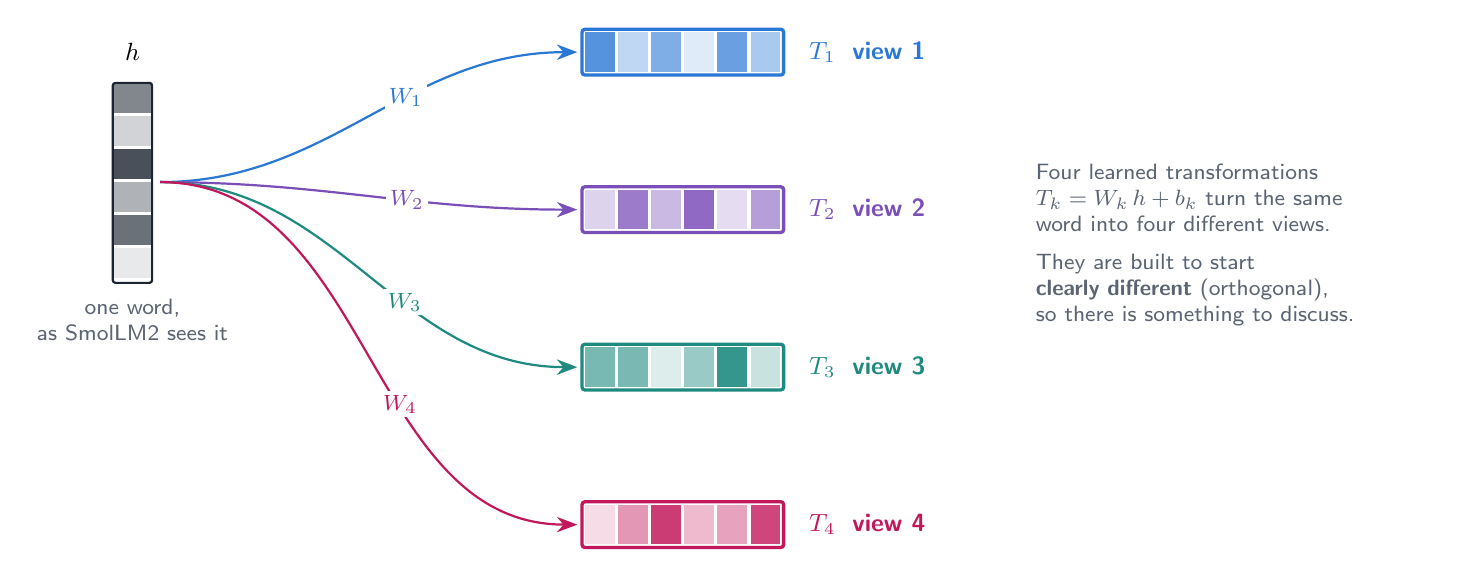
\begin{tikzpicture}
  \def\cells#1#2#3{% x, colour, list of shades
    \foreach \s [count=\i] in {#3} { \fill[#2!\s] (#1,{2.1-\i*0.42}) rectangle ++(0.5,0.38); }
    \draw[ink,thick,rounded corners=1pt] (#1,-0.48) rectangle ++(0.5,2.54);}
  \cells{0}{ink}{55,20,80,35,65,10}
  \node[font=\small\bfseries] at (0.25,2.45) {$h$};
  \node[lab] at (0.25,-0.95) {one word,\\as SmolLM2 sees it};
  \foreach \c/\sh/\y/\k in {r1/{80,30,60,15,70,40}/3.0/1, r2/{25,75,40,85,20,55}/1.0/2, r3/{60,60,15,45,90,25}/-1.0/3, r4/{15,45,85,30,40,80}/-3.0/4} {
    \begin{scope}[shift={(6,\y-0.8)}]
      \foreach \s [count=\i] in \sh { \fill[\c!\s] ({\i*0.42-0.42},0) rectangle ++(0.38,0.5); }
      \draw[\c,very thick,rounded corners=1pt] (-0.04,-0.04) rectangle ({6*0.42},0.54);
      \node[font=\small\bfseries,color=\c,anchor=west] at ({6*0.42+0.2},0.25) {$T_{\k}$ \;view \k};
    \end{scope}
    \draw[->,thick,\c] (0.6,0.8) to[out=0,in=180] node[pos=0.6,fill=white,inner sep=1.5pt,font=\footnotesize,text=\c]{$W_{\k}$} (5.9,\y-0.55);
  }
  \node[lab,anchor=west,text width=5.2cm,align=left] at (11.6,0.0) {Four learned transformations\\$T_k = W_k\,h + b_k$ turn the same\\word into four different views.\\[4pt]They are built to start\\\textbf{clearly different} (orthogonal),\\so there is something to discuss.};
\end{tikzpicture}

% ------------------------------------------------------------------ 3 step 2: discussion round
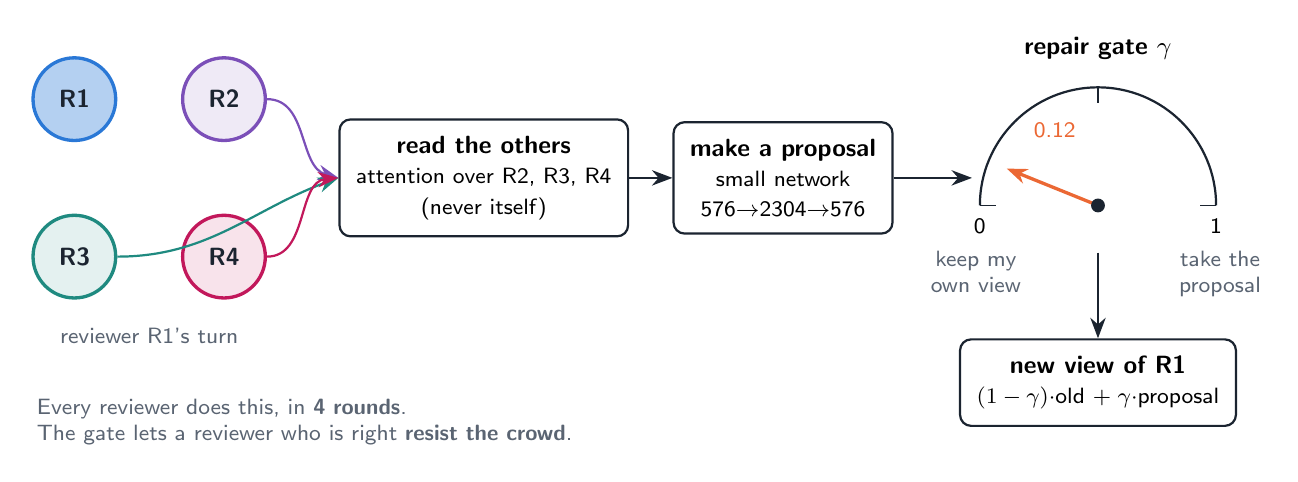
\begin{tikzpicture}
  \node[rev=r1,fill=r1!35] (a) at (0,1.0) {R1};
  \node[rev=r2] (b) at (1.9,1.0) {R2};
  \node[rev=r3] (c) at (0,-1.0) {R3};
  \node[rev=r4] (d) at (1.9,-1.0) {R4};
  \node[lab] at (0.95,-2.0) {reviewer R1's turn};
  \node[box,minimum width=2.6cm,minimum height=1.2cm] (read) at (5.2,0) {\textbf{read the others}\\{\footnotesize attention over R2, R3, R4}\\{\footnotesize (never itself)}};
  \draw[->,thick,r2] (b) to[out=0,in=165] (read.west);
  \draw[->,thick,r3] (c) to[out=0,in=200] (read.west);
  \draw[->,thick,r4] (d) to[out=0,in=185] (read.west);
  \node[box,minimum width=2.4cm,minimum height=1.2cm] (prop) at (9.0,0) {\textbf{make a proposal}\\{\footnotesize small network}\\{\footnotesize 576$\rightarrow$2304$\rightarrow$576}};
  \draw[flow] (read) -- (prop);
  % dial
  \begin{scope}[shift={(13.0,-0.35)}]
    \draw[ink,thick] (-1.5,0) arc (180:0:1.5);
    \foreach \a/\t in {180/0, 90/0.5, 0/1} { \draw[ink] ({1.5*cos(\a)},{1.5*sin(\a)}) -- ({1.3*cos(\a)},{1.3*sin(\a)}); }
    \node[font=\footnotesize,anchor=north] at (-1.5,-0.05) {0};
    \node[font=\footnotesize,anchor=north] at (1.5,-0.05) {1};
    \draw[->,very thick,lorange] (0,0) -- ({1.25*cos(158)},{1.25*sin(158)});
    \fill[ink] (0,0) circle (2.5pt);
    \node[font=\small\bfseries] at (0,2.0) {repair gate $\gamma$};
    \node[lab,anchor=north] at (-1.55,-0.45) {keep my\\own view};
    \node[lab,anchor=north] at (1.55,-0.45) {take the\\proposal};
    \node[font=\footnotesize,color=lorange] at (-0.55,0.95) {0.12};
  \end{scope}
  \draw[flow] (prop) -- (11.4,0);
  \node[box,minimum width=2.5cm] (new) at (13.0,-2.6) {\textbf{new view of R1}\\{\footnotesize $(1-\gamma)\cdot$old $+\;\gamma\cdot$proposal}};
  \draw[flow] (13.0,-0.95) -- (new);
  \node[lab,anchor=west,text width=7cm,align=left] at (-0.6,-3.1) {Every reviewer does this, in \textbf{4 rounds}.\\The gate lets a reviewer who is right \textbf{resist the crowd}.};
\end{tikzpicture}

% ------------------------------------------------------------------ 4 step 3: staying grounded
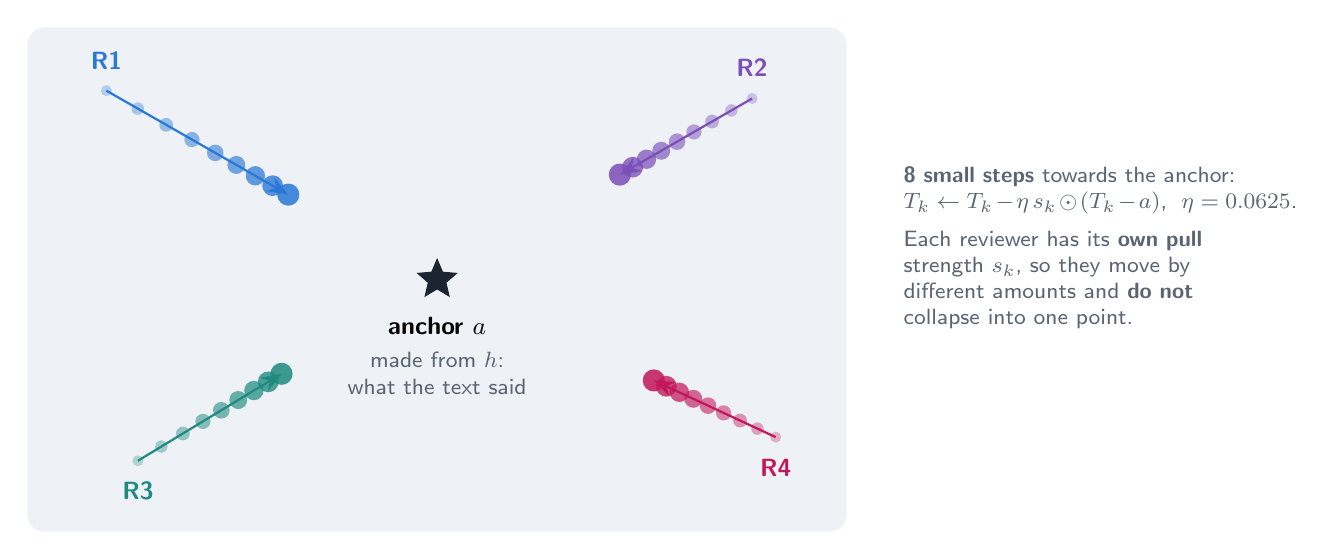
\begin{tikzpicture}
  \fill[tint,rounded corners=6pt] (-5.2,-3.2) rectangle (5.2,3.2);
  \node[star,star points=5,star point ratio=2.2,fill=ink,minimum size=0.55cm,inner sep=0] (anc) at (0,0) {};
  \node[font=\small\bfseries,anchor=north] at (0,-0.35) {anchor $a$};
  \node[lab,anchor=north] at (0,-0.8) {made from $h$: \\what the text said};
  \foreach \c/\x/\y/\f in {r1/-4.2/2.4/0.55, r2/4.0/2.3/0.42, r3/-3.8/-2.3/0.48, r4/4.3/-2.0/0.36} {
    \foreach \i in {0,...,8} {
      \pgfmathsetmacro{\t}{1-(1-\f)^(\i/8)}
      \pgfmathsetmacro{\px}{\x*(1-\t*1.0)}
      \pgfmathsetmacro{\py}{\y*(1-\t*1.0)}
      \fill[\c, opacity={0.3+0.07*\i}] (\px,\py) circle ({2pt+0.25pt*\i});
    }
    \pgfmathsetmacro{\ex}{\x*(1-\f)} \pgfmathsetmacro{\ey}{\y*(1-\f)}
    \draw[->,thick,\c] (\x,\y) -- (\ex,\ey);
  }
  \node[font=\small\bfseries,color=r1,anchor=south] at (-4.2,2.55) {R1};
  \node[font=\small\bfseries,color=r2,anchor=south] at (4.0,2.45) {R2};
  \node[font=\small\bfseries,color=r3,anchor=north] at (-3.8,-2.45) {R3};
  \node[font=\small\bfseries,color=r4,anchor=north] at (4.3,-2.15) {R4};
  \node[lab,anchor=west,text width=5.0cm,align=left] at (5.8,0.4) {\textbf{8 small steps} towards the anchor:\\$T_k \leftarrow T_k - \eta\, s_k\odot(T_k-a)$,\; $\eta=0.0625$.\\[4pt]Each reviewer has its \textbf{own pull}\\strength $s_k$, so they move by\\different amounts and \textbf{do not}\\collapse into one point.};
\end{tikzpicture}

% ------------------------------------------------------------------ 5 step 4: verdict and gate
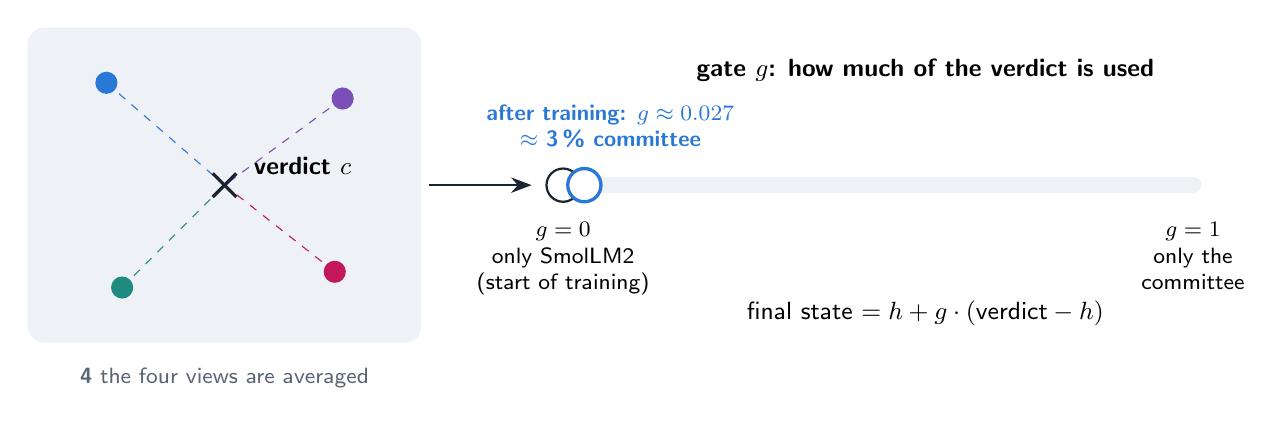
\begin{tikzpicture}
  \fill[tint,rounded corners=6pt] (-0.4,-1.9) rectangle (4.6,2.1);
  \foreach \c/\x/\y in {r1/0.6/1.4, r2/3.6/1.2, r3/0.8/-1.2, r4/3.5/-1.0} {
    \fill[\c] (\x,\y) circle (4pt);
    \draw[thin,\c,dashed] (\x,\y) -- (2.1,0.1);
  }
  \draw[ink,very thick] (1.95,-0.05) -- (2.25,0.25); \draw[ink,very thick] (1.95,0.25) -- (2.25,-0.05);
  \node[font=\small\bfseries,anchor=west] at (2.35,0.35) {verdict $c$};
  \node[lab] at (2.1,-2.35) {\textbf{4} the four views are averaged};
  \draw[flow] (4.7,0.1) -- (6.0,0.1);
  % slider
  \begin{scope}[shift={(6.4,0)}]
    \draw[line width=6pt,tint,line cap=round] (0,0.1) -- (8,0.1);
    \draw[line width=6pt,lblue,line cap=round] (0,0.1) -- (0.35,0.1);
    \fill[white,draw=ink,thick] (0,0.1) circle (6pt);
    \fill[white,draw=lblue,very thick] (0.27,0.1) circle (6pt);
    \node[font=\footnotesize,anchor=north,align=center] at (0,-0.25) {$g = 0$\\only SmolLM2\\(start of training)};
    \node[font=\footnotesize,anchor=north,align=center] at (8,-0.25) {$g = 1$\\only the\\committee};
    \node[font=\footnotesize\bfseries,color=lblue,anchor=south,align=center] at (0.6,0.45) {after training: $g \approx 0.027$\\$\approx$ 3\,\% committee};
    \node[font=\small\bfseries,anchor=south] at (4.6,1.3) {gate $g$: how much of the verdict is used};
    \node[font=\small,anchor=north] at (4.6,-1.25) {final state $= h + g\cdot(\text{verdict} - h)$};
  \end{scope}
\end{tikzpicture}

% ------------------------------------------------------------------ 6 spread floor
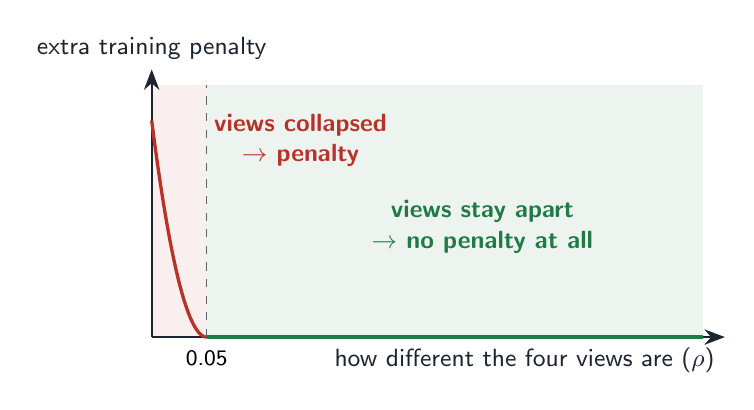
\begin{tikzpicture}[x=1.4cm,y=1.0cm]
  \fill[lred!8] (0,0) rectangle (0.5,3.2);
  \fill[lgreen!8] (0.5,0) rectangle (5,3.2);
  \draw[->,thick,ink] (0,0) -- (5.2,0) node[below left,font=\small]{how different the four views are ($\rho$)};
  \draw[->,thick,ink] (0,0) -- (0,3.4) node[above,font=\small]{extra training penalty};
  \draw[very thick,lred,domain=0:0.5,samples=40] plot (\x,{11*(0.5-\x)^2});
  \draw[very thick,lgreen] (0.5,0) -- (5,0);
  \draw[dashed,muted] (0.5,0) -- (0.5,3.2);
  \node[font=\footnotesize,anchor=north] at (0.5,-0.05) {0.05};
  \node[font=\small\bfseries,color=lred,align=center] at (1.35,2.5) {views collapsed\\$\rightarrow$ penalty};
  \node[font=\small\bfseries,color=lgreen,align=center] at (3.0,1.4) {views stay apart\\$\rightarrow$ no penalty at all};
\end{tikzpicture}

% ------------------------------------------------------------------ 7 threshold shift (calibration)
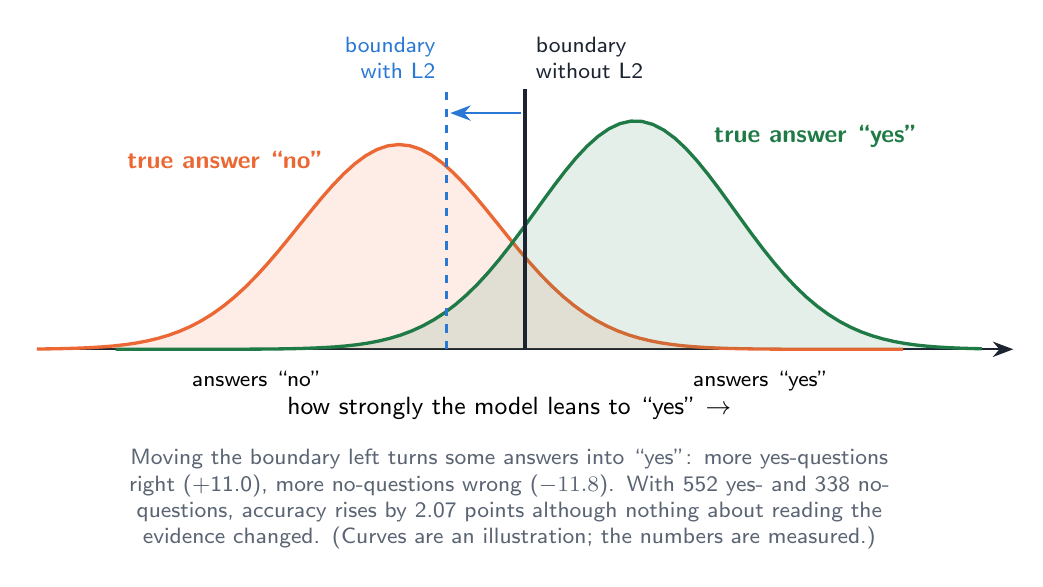
\begin{tikzpicture}[x=1cm,y=1cm]
  \draw[->,thick,ink] (-6,0) -- (6.4,0);
  \node[font=\small] at (0,-0.75) {how strongly the model leans to ``yes'' $\rightarrow$};
  \draw[very thick,lorange,domain=-6:5,samples=80,fill=lorange,fill opacity=0.12] plot (\x,{2.6*exp(-((\x+1.4)^2)/3.2)});
  \draw[very thick,lgreen,domain=-5:6,samples=80,fill=lgreen,fill opacity=0.12] plot (\x,{2.9*exp(-((\x-1.6)^2)/3.2)});
  \node[font=\small\bfseries,color=lorange] at (-3.6,2.4) {true answer ``no''};
  \node[font=\small\bfseries,color=lgreen] at (3.9,2.7) {true answer ``yes''};
  \draw[very thick,ink] (0.2,0) -- (0.2,3.3) node[above right,font=\footnotesize,align=left]{boundary\\without L2};
  \draw[very thick,dashed,lblue] (-0.8,0) -- (-0.8,3.3) node[above left,font=\footnotesize,align=right,text=lblue]{boundary\\with L2};
  \draw[<-,thick,lblue] (-0.75,3.0) -- (0.15,3.0);
  \node[font=\footnotesize,anchor=north,align=center] at (-3.2,-0.15) {answers ``no''};
  \node[font=\footnotesize,anchor=north,align=center] at (3.2,-0.15) {answers ``yes''};
  \node[lab,anchor=north,text width=12cm] at (0,-1.15) {Moving the boundary left turns some answers into ``yes'': more yes-questions right (+11.0), more no-questions wrong ($-11.8$). With 552 yes- and 338 no-questions, accuracy rises by 2.07 points although nothing about reading the evidence changed. (Curves are an illustration; the numbers are measured.)};
\end{tikzpicture}

% ------------------------------------------------------------------ 8 expectation vs result
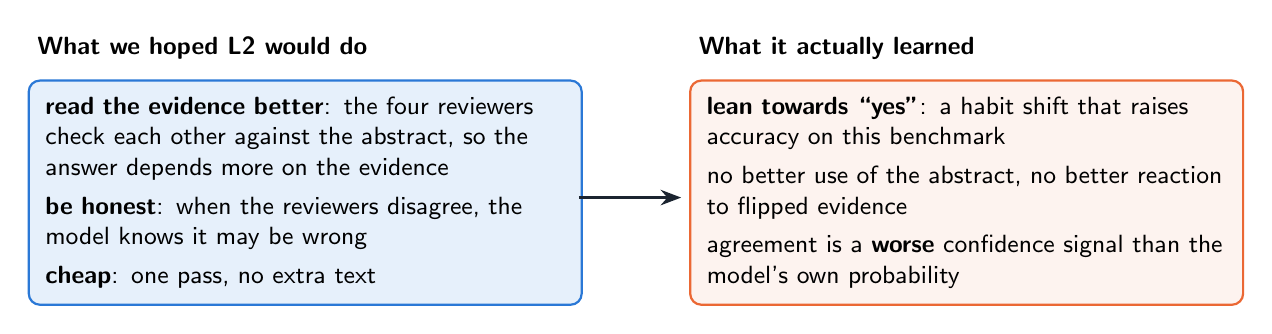
\begin{tikzpicture}
  \node[font=\small\bfseries,anchor=west] at (0,4.3) {What we hoped L2 would do};
  \node[font=\small\bfseries,anchor=west] at (8.4,4.3) {What it actually learned};
  \node[box,soft,text width=6.6cm,align=left,anchor=north west] at (0,3.9) {\textbf{read the evidence better}: the four reviewers check each other against the abstract, so the answer depends more on the evidence\\[3pt]\textbf{be honest}: when the reviewers disagree, the model knows it may be wrong\\[3pt]\textbf{cheap}: one pass, no extra text};
  \node[box,draw=lorange,fill=lorange!8,text width=6.6cm,align=left,anchor=north west] at (8.4,3.9) {\textbf{lean towards ``yes''}: a habit shift that raises accuracy on this benchmark\\[3pt]no better use of the abstract, no better reaction to flipped evidence\\[3pt]agreement is a \textbf{worse} confidence signal than the model's own probability};
  \draw[->,very thick,ink] (7.0,2.4) -- (8.3,2.4);
\end{tikzpicture}

\end{document}
